\documentclass{article}

\usepackage{graphicx}

\pagestyle{headings}

\title{DETAIL DESIGN}
\author{WANG Chen, 2015213086, wangchen@bupt.edu.cn}
\date{\today}

\begin{document}

\maketitle

\tableofcontents

\newpage
\section{INTRODUCTION}

This is a detail design document for a simple shell program named msh.
The shell program is a course assignment in \emph{Advanced Programming in the UNIX Environment}.
It will make us have a deeper understanding in UNIX C programming, after we finish this program.
This document include LOGIC FLOW and FUNCTIONS DESIGN.
LOGIC FLOW show all functions we defined and their relation.
FUNCTIONS DESIGN illustrate how we build these functions, it include the return type, parameters and variables declaration, built-in function we used.

\newpage
\section{LOGIC FLOW}

\begin{figure}[h]
\centering
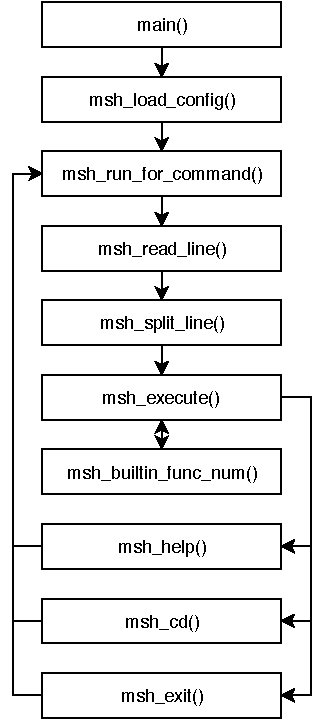
\includegraphics[scale=0.85]{fig/ShellLogicFlow.pdf}
\caption{Logic flow of the shell}
\label{logicFlow}
\end{figure}

Figure \ref{logicFlow} show logic flow of the shell program.
After user input "\verb|./msh|" in terminal to run the program, \verb|main()| function will be started, and running configuration will be loaded by \verb|msh_load_config()| function.
The shell will set command prompt according running configuration.
Then the shell will wait for input from users.
\verb|msh_read_line()| will get the input from users, and store it.
And those input, will be split to some arguments by \verb|msh_split_line()| according to specific delim.
Next, the shell will use this arguments to run command.
Normally, \verb|args[0]| is the command name which users want to run, and the other arguments are taken as the parameters of the command.
\verb|msh_help()|, \verb|msh_cd()| and \verb|msh_exit()| are built-in functions of the shell program.
\verb|msh_builtin_func_num()| is used to count the number of built-in functions for calling them.
When \verb|msh| try to run the command, it will judge whether it is a built-in function or not.
If the command is a built-in function, it will run the corresponding function in \verb|msh|.
Otherwise, it will use \verb|execvp()| which is provided in UNIX to run the command.


\newpage
\section{DEPENDENCY}

\begin{figure}[h]
\centering
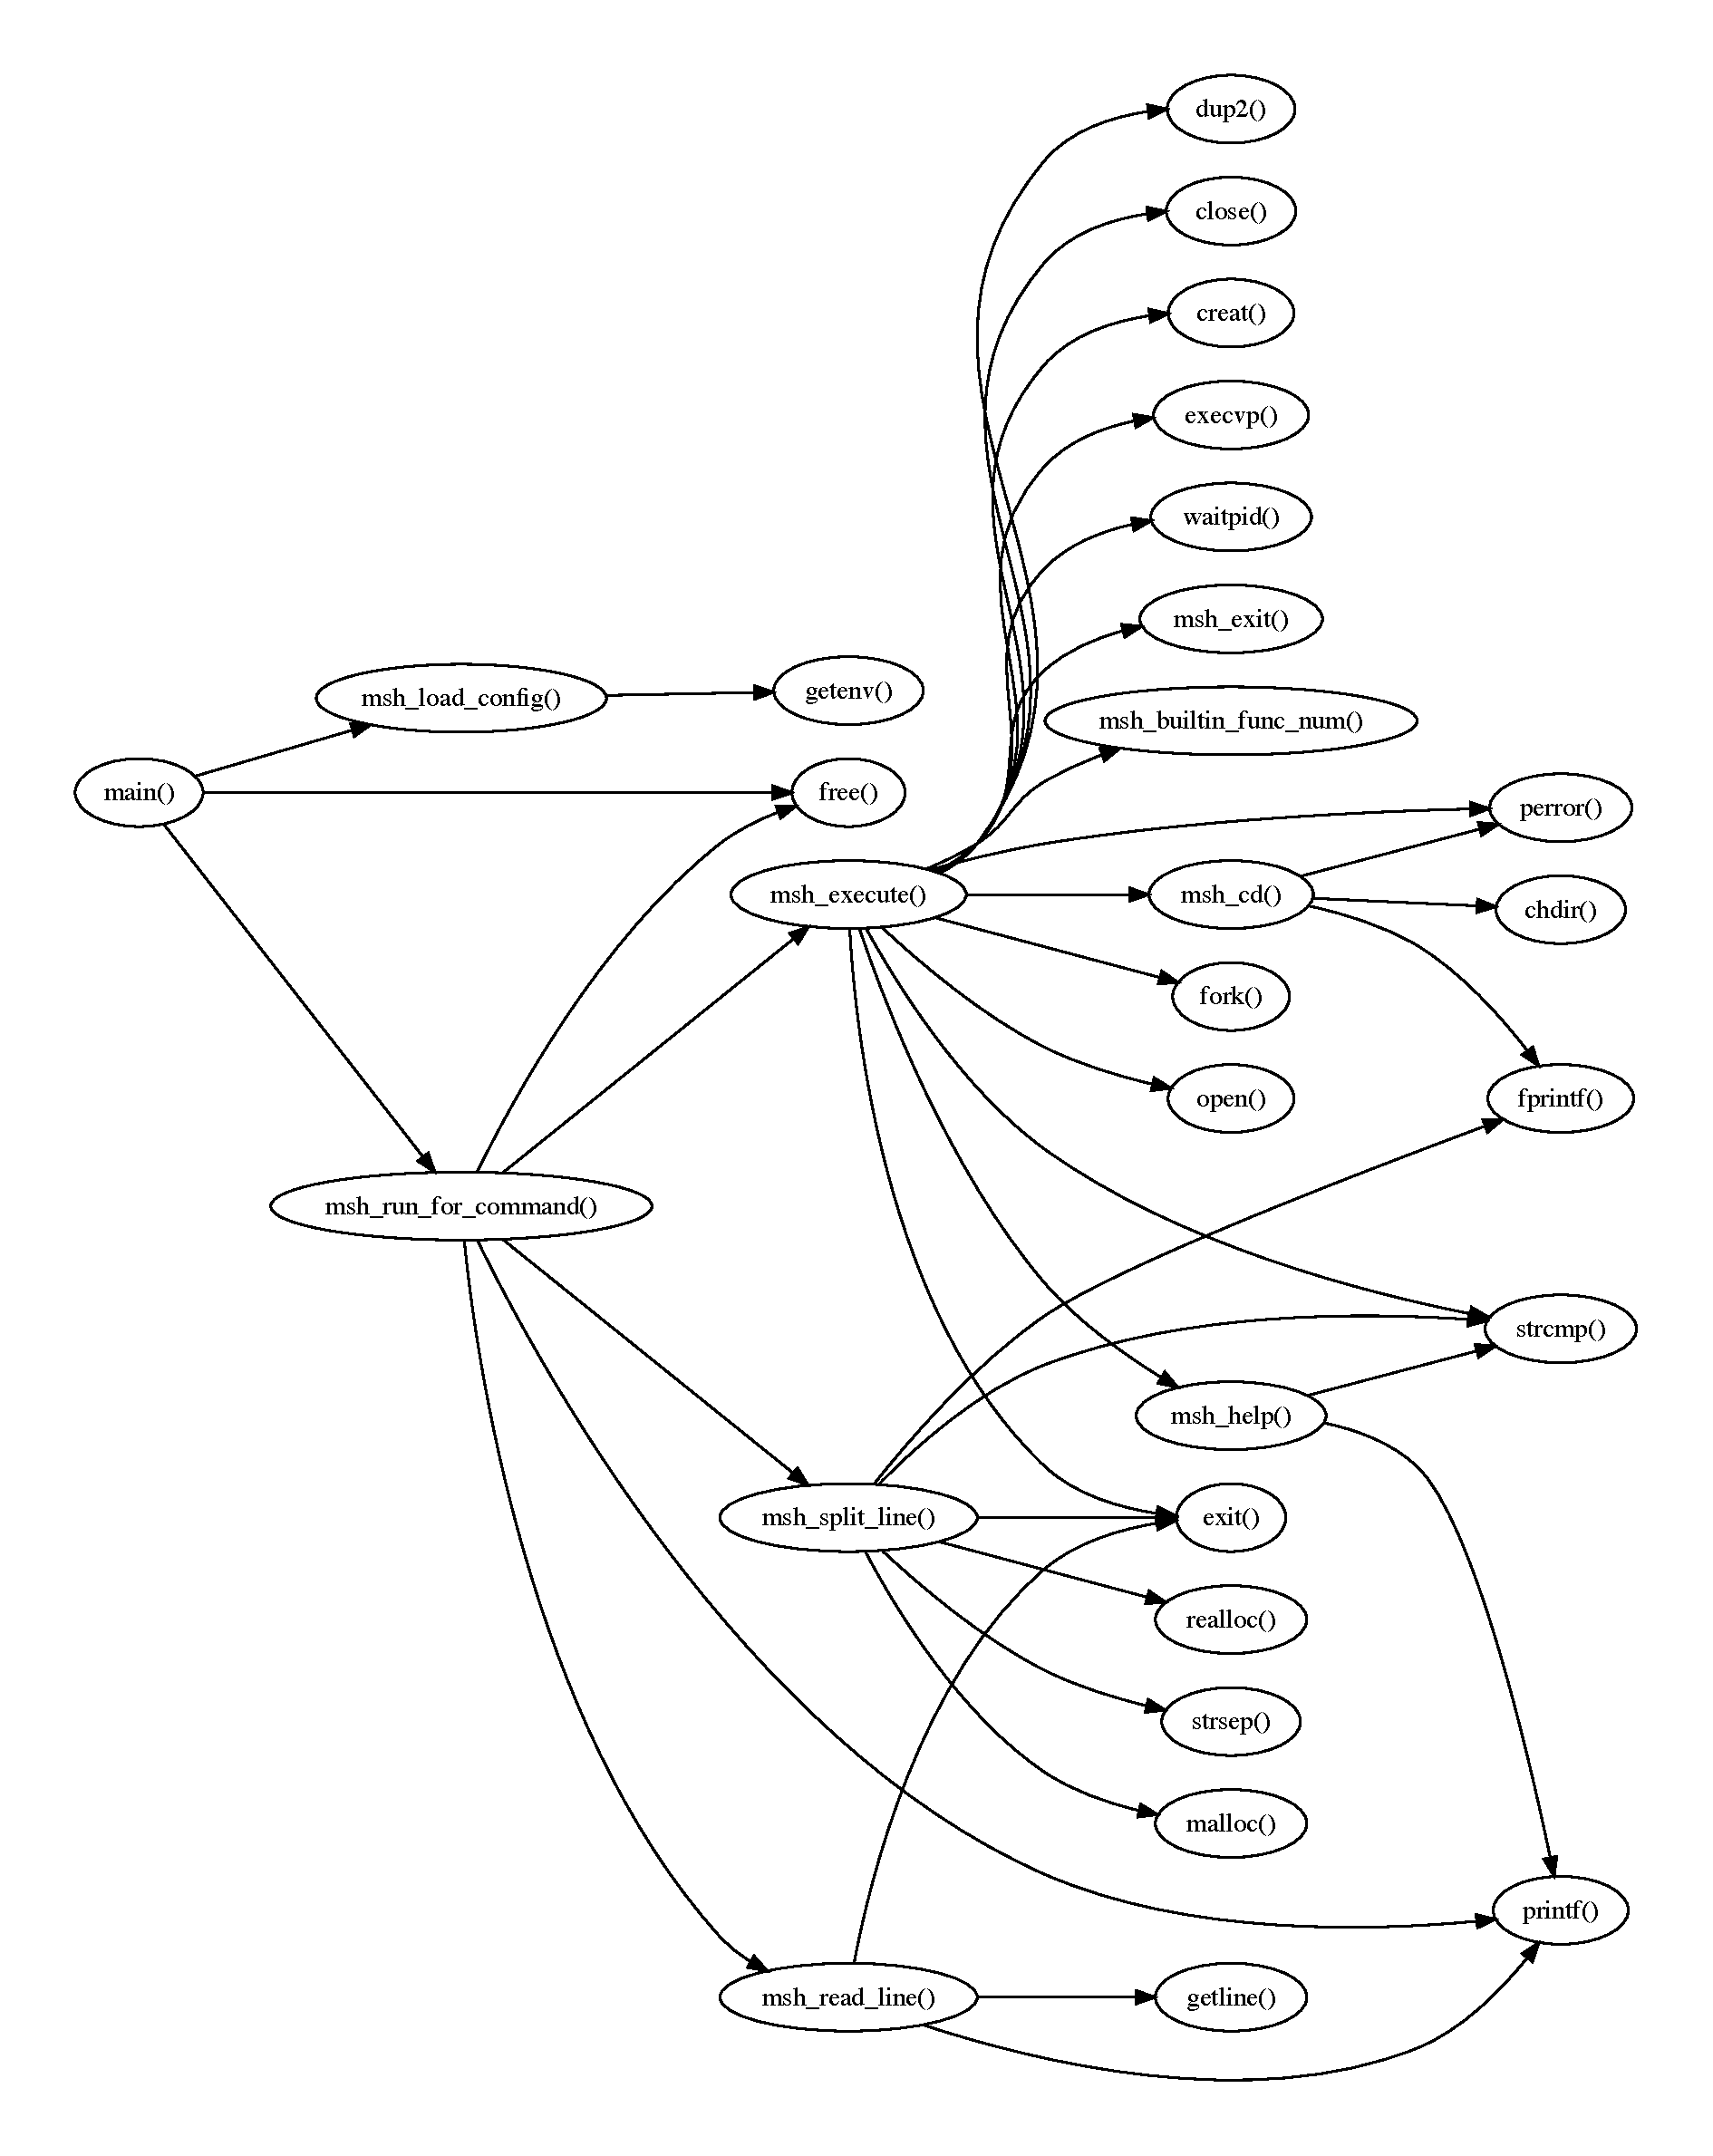
\includegraphics[scale=0.3]{fig/ShellDependency.pdf}
\caption{Dependency of the shell}
\label{dependency}
\end{figure}

Figure \ref{dependency} show the dependencies in the shell program.
It can help us to understand the shell program better.
The level of functions become lower from left to right.

\newpage
\section{FUNCTIONS DESIGN}
\subsection{main}
\begin{itemize}
\item Description

This is entry of program, includes 2 functions, \verb|msh_load_config| and \verb|msh_run_for_command|.

\item Return Type

\verb|int|

\item Parameters

\verb|int argc, char **argv|

\item Variables

\verb|void|

\item Library Used

\verb|<stdlib.h>|: \verb|free()|
\end{itemize}

\subsection{msh\_load\_config}
\begin{itemize}
\item Description

This function is used to load running configuration of the shell.
User can modify the environment variable named "msh\_cp" to change the command prompt.

\item Return Type

\verb|void|

\item Parameters

\verb|void|

\item Variables

\verb|void|

\item Library Used

\verb|<stdlib.h>|: \verb|getenv()|
\end{itemize}

\subsection{msh\_run\_for\_command}
\begin{itemize}
\item Description

This function is used to wait for input from user. The command prompt is presented in here. Indicator of input and output redirection are reseted here.

\item Return Type

\verb|void|

\item Parameters

\verb|void|

\item Variables

\verb|char *line|, \verb|char **args|, \verb|int status|

\item Library Used

\verb|<stdio.h>|: \verb|printf()|

\verb|<stdlib.h>|: \verb|free()|
\end{itemize}

\subsection{msh\_read\_line}
\begin{itemize}
\item Description

This function is used to read the input of user from keyboard.

\item Return Type

\verb|char *|

\item Parameters

\verb|void|

\item Variables

\verb|char *line|, \verb|size_t n|

\item Library Used

\verb|<stdio.h>|: \verb|getline()|, \verb|printf()|

\verb|<stdlib.h>|: \verb|exit()|
\end{itemize}

\subsection{msh\_split\_line}
\begin{itemize}
\item Description

This function is used to split line into some arguments according to specific delim.

\item Return Type

\verb|char **|

\item Parameters

\verb|char *line|

\item Variables

\verb|int bufsize|, \verb|cur_arg_pos|, \verb|char **args|, \verb|char *delim|, \verb|char *arg|

\item Library Used

\verb|<stdlib.h>|: \verb|malloc()|, \verb|realloc()|, \verb|exit()|

\verb|<stdio.h>|: \verb|fprintf()|

\verb|<string.h>|: \verb|strsep()|, \verb|strcmp()|
\end{itemize}

\subsection{msh\_execute}
\begin{itemize}
\item Description

This function is used to execute command.

\item Return Type

\verb|int|

\item Parameters

\verb|char **args|

\item Variables

\verb|int i|, \verb|int status|, \verb|int fd|, \verb|pid_t pid|

\item Library Used

\verb|<unistd.h>|: \verb|pid_t|, \verb|fork()|, \verb|dup2()|,

\verb|<string.h>|: \verb|strcmp()|

\verb|<fcntl.h>|: \verb|open()|, \verb|close()|, \verb|creat()|

\verb|<stdlib.h>|: \verb|execvp()|, \verb|exit()|

\verb|<stdio.h>|: \verb|perror()|

\verb|<sys/wait.h>|: \verb|waitpid()|
\end{itemize}

\subsection{msh\_exit}
\begin{itemize}
\item Description

This function is a built-in function, used to close the shell.

\item Return Type

\verb|int|

\item Parameters

\verb|char **args|

\item Variables

\verb|void|

\item Library Used

\verb|void|
\end{itemize}

\subsection{msh\_help}
\begin{itemize}
\item Description

This function is a built-in function, and it provides some information about the shell.

\item Return Type

\verb|int|

\item Parameters

\verb|char **args|

\item Variables

\verb|void|

\item Library Used

\verb|<stdio.h>|: \verb|printf()|

\verb|<string.h>|: \verb|strcmp()|
\end{itemize}

\subsection{msh\_cd}
\begin{itemize}
\item Description

This function is a built-in function, used to change current dir.

\item Return Type

\verb|int|

\item Parameters

\verb|char **args|

\item Variables

\verb|void|

\item Library Used

\verb|<unistd.h>|: \verb|chdir()|

\verb|<stdio.h>|: \verb|fprintf()|, \verb|perror()|

\end{itemize}

\subsection{msh\_builtin\_func\_num}
\begin{itemize}
\item Description

This function is used to count the number of built-in functions.

\item Return Type

\verb|int|

\item Parameters

\verb|void|

\item Variables

\verb|void|

\item Library Used

\verb|void|
\end{itemize}

\newpage
\section{DEVELOPMENT ENVIRONMENT}

\begin{itemize}
\item Hardware: Macbook pro 2018
\item System: Mac OS 10.14.4
\item Code Software: Visual Studio Code
\item Compiler: GCC 4.2.1
\end{itemize}

\end{document}